%% LyX 2.0.6 created this file.  For more info, see http://www.lyx.org/.
%% Do not edit unless you really know what you are doing.
\documentclass[10pt]{beamer}\usepackage[]{graphicx}\usepackage[]{color}
%% maxwidth is the original width if it is less than linewidth
%% otherwise use linewidth (to make sure the graphics do not exceed the margin)
\makeatletter
\def\maxwidth{ %
  \ifdim\Gin@nat@width>\linewidth
    \linewidth
  \else
    \Gin@nat@width
  \fi
}
\makeatother

\definecolor{fgcolor}{rgb}{0.345, 0.345, 0.345}
\newcommand{\hlnum}[1]{\textcolor[rgb]{0.686,0.059,0.569}{#1}}%
\newcommand{\hlstr}[1]{\textcolor[rgb]{0.192,0.494,0.8}{#1}}%
\newcommand{\hlcom}[1]{\textcolor[rgb]{0.678,0.584,0.686}{\textit{#1}}}%
\newcommand{\hlopt}[1]{\textcolor[rgb]{0,0,0}{#1}}%
\newcommand{\hlstd}[1]{\textcolor[rgb]{0.345,0.345,0.345}{#1}}%
\newcommand{\hlkwa}[1]{\textcolor[rgb]{0.161,0.373,0.58}{\textbf{#1}}}%
\newcommand{\hlkwb}[1]{\textcolor[rgb]{0.69,0.353,0.396}{#1}}%
\newcommand{\hlkwc}[1]{\textcolor[rgb]{0.333,0.667,0.333}{#1}}%
\newcommand{\hlkwd}[1]{\textcolor[rgb]{0.737,0.353,0.396}{\textbf{#1}}}%

\usepackage{framed}
\makeatletter
\newenvironment{kframe}{%
 \def\at@end@of@kframe{}%
 \ifinner\ifhmode%
  \def\at@end@of@kframe{\end{minipage}}%
  \begin{minipage}{\columnwidth}%
 \fi\fi%
 \def\FrameCommand##1{\hskip\@totalleftmargin \hskip-\fboxsep
 \colorbox{shadecolor}{##1}\hskip-\fboxsep
     % There is no \\@totalrightmargin, so:
     \hskip-\linewidth \hskip-\@totalleftmargin \hskip\columnwidth}%
 \MakeFramed {\advance\hsize-\width
   \@totalleftmargin\z@ \linewidth\hsize
   \@setminipage}}%
 {\par\unskip\endMakeFramed%
 \at@end@of@kframe}
\makeatother

\definecolor{shadecolor}{rgb}{.97, .97, .97}
\definecolor{messagecolor}{rgb}{0, 0, 0}
\definecolor{warningcolor}{rgb}{1, 0, 1}
\definecolor{errorcolor}{rgb}{1, 0, 0}
\newenvironment{knitrout}{}{} % an empty environment to be redefined in TeX

\usepackage{alltt}
\usepackage[T1]{fontenc}
\usepackage[normalem]{ulem}
\usepackage{graphicx, mwe, caption}
\usepackage{comment}
\usepackage{epigraph}
\usepackage{amsmath}
\setcounter{secnumdepth}{3}
\setcounter{tocdepth}{3}
\usepackage{url}
\ifx\hypersetup\undefined
  \AtBeginDocument{%
    \hypersetup{unicode=true,pdfusetitle,
 bookmarks=true,bookmarksnumbered=false,bookmarksopen=false,
 breaklinks=false,pdfborder={0 0 0},backref=false,colorlinks=false}
  }
\else
  \hypersetup{unicode=true,pdfusetitle,
 bookmarks=true,bookmarksnumbered=false,bookmarksopen=false,
 breaklinks=false,pdfborder={0 0 0},backref=false,colorlinks=false}
\fi
\usepackage{breakurl}

\makeatletter

%%%%%%%%%%%%%%%%%%%%%%%%%%%%%% LyX specific LaTeX commands.
\providecommand{\LyX}{\texorpdfstring%
  {L\kern-.1667em\lower.25em\hbox{Y}\kern-.125emX\@}
  {LyX}}

%%%%%%%%%%%%%%%%%%%%%%%%%%%%%% Textclass specific LaTeX commands.
 % this default might be overridden by plain title style
 \newcommand\makebeamertitle{\frame{\maketitle}}%
 \AtBeginDocument{
   \let\origtableofcontents=\tableofcontents
   \def\tableofcontents{\@ifnextchar[{\origtableofcontents}{\gobbletableofcontents}}
   \def\gobbletableofcontents#1{\origtableofcontents}
 }
 \def\lyxframeend{} % In case there is a superfluous frame end
 \long\def\lyxframe#1{\@lyxframe#1\@lyxframestop}%
 \def\@lyxframe{\@ifnextchar<{\@@lyxframe}{\@@lyxframe<*>}}%
 \def\@@lyxframe<#1>{\@ifnextchar[{\@@@lyxframe<#1>}{\@@@lyxframe<#1>[]}}
 \def\@@@lyxframe<#1>[{\@ifnextchar<{\@@@@@lyxframe<#1>[}{\@@@@lyxframe<#1>[<*>][}}
 \def\@@@@@lyxframe<#1>[#2]{\@ifnextchar[{\@@@@lyxframe<#1>[#2]}{\@@@@lyxframe<#1>[#2][]}}
 \long\def\@@@@lyxframe<#1>[#2][#3]#4\@lyxframestop#5\lyxframeend{%
   \frame<#1>[#2][#3]{\frametitle{#4}#5}}

%%%%%%%%%%%%%%%%%%%%%%%%%%%%%% User specified LaTeX commands.
%\usetheme{PaloAlto}
\usepackage{etex}
\mode<presentation>
\usetheme{Warsaw}
\usepackage{wrapfig}
\usepackage{subcaption}

\useinnertheme{rectangles}
\setbeamertemplate{navigation symbols}{}
\setbeamertemplate{footline}[frame number]
\setbeamertemplate{caption}[numbered]
\addtobeamertemplate{headline}{}{\vskip2pt}
%\usecolortheme{beaver}

\newcounter{saveenumi}
\newcommand{\seti}{\setcounter{saveenumi}{\value{enumi}}}
\newcommand{\conti}{\setcounter{enumi}{\value{saveenumi}}}

\resetcounteronoverlays{saveenumi}

\makeatother
\IfFileExists{upquote.sty}{\usepackage{upquote}}{}

\begin{document}








\title[Reproducible Research (RR)]{Reproducible Research (RR) and \emph{Biostatistics}}


\author{Sahir Rai Bhatnagar%
\thanks{McGill Biostats Reading Group%
}}

\makebeamertitle

\lyxframeend{}


\lyxframeend{}\lyxframe{Disclaimer}
\begin{itemize}
\item I will ask you alot of questions
\item Your participation is necessary for this to be useful
\item Interrupt me often
\item This is a \sout{reading} discussion group
\end{itemize}

\lyxframeend{}\lyxframe{Outline}
\begin{itemize}
\item Some motivating examples
\item The problem
\item A solution
\end{itemize}

%%%%%%%%%%%%%%%%%%%%%%%%%%%%%%%%%%%%%%%%%%%%%%%%%%%%%%%%%%%%%%%%%%%%%%%%%%%%%%%%%%%%%%%%%%%%%
%%%%%%%%%%%%%%%%%%%%%%%%%%%%%%%%%%%%%%%%%%%%%%%%%%%%%%%%%%%%%%%%%%%%%%%%%%%%%%%%%%%%%%%%%%%%%
%%%%%%%%%%%%%%%%%%%%%%%%%%%%%%%%%%%%%%%%%%%%%%%%%%%%%%%%%%%%%%%%%%%%%%%%%%%%%%%%%%%%%%%%%%%%%
\lyxframeend{}\section{Introduction}

\lyxframeend{}\subsection{What is RR?}
\begin{frame}

\frametitle{What is Science Anyway?}

\pause
\begin{block}{According to the American Physical Society:}
\emph{Science is the systematic enterprise of gathering knowledge about the universe and organizing and condensing that knowledge into \textbf{testable} laws and theories. The success and credibility of science are anchored in the \textbf{willingness} of scientists to \textbf{expose their ideas} and results to \textbf{independent testing} and \textbf{replication} by other scientists}
\end{block}

\end{frame}

%%%%%%%%%%%%%%%%%%%%%%%%%%%%%%%%%%%%%%%%%%%%%%%%%%%%%%%%%%%%%%%%%%%%%%%%%%%%%%%%%%%%%%%%%%%%%
\begin{frame}

\frametitle{A Minimum Standard to Verify Scientific Findings}

\pause
\begin{block}{Reproducible Research in Computational Sciences}
\emph{The data and the code used to make a finding are available and they are sufficient for an independent researcher to recreate the finding}
\end{block}

\end{frame}

%%%%%%%%%%%%%%%%%%%%%%%%%%%%%%%%%%%%%%%%%%%%%%%%%%%%%%%%%%%%%%%%%%%%%%%%%%%%%%%%%%%%%%%%%%%%%
%%%%%%%%%%%%%%%%%%%%%%%%%%%%%%%%%%%%%%%%%%%%%%%%%%%%%%%%%%%%%%%%%%%%%%%%%%%%%%%%%%%%%%%%%%%%%

\lyxframeend{}\subsection{Why should we care about RR?}
\begin{frame}

\frametitle{For Science}

\pause
\begin{enumerate}
\item Findings cannot be considered genuine contributions until verified through \textcolor{blue}{independent replication} (whenever possible)
\pause
\begin{itemize}
\item \emph{``Don't worry, the car runs perfectly... Give me \$10k, and I give you my word''}
\end{itemize}
\pause
\vspace{0.3in}
\item Enables the \textcolor{blue}{cumulative growth} of future scientific knowledge
\pause
\begin{itemize}
\item \emph{Stop wasting public funds on something that has already been done}
\end{itemize}
\end{enumerate}

\end{frame}

%%%%%%%%%%%%%%%%%%%%%%%%%%%%%%%%%%%%%%%%%%%%%%%%%%%%%%%%%%%%%%%%%%%%%%%%%%%%%%%%%%%%%%%%%%%%%
\begin{frame}
\frametitle{For You}

\pause
\begin{enumerate}

\item \textbf{Better work habits}
\begin{itemize}
\item \emph{Who cares if no one else is watching?}
\end{itemize}

\vspace{0.2in}
\pause
\item \textbf{Better teamwork}
\begin{itemize}
\item \emph{Bring current and future collaborators upto speed with ease}
\end{itemize}

\vspace{0.2in}
\pause
\item \textbf{Changes are easier}
\begin{itemize}
\item \emph{No research process is linear}
\end{itemize}

\vspace{0.2in}
\pause
\item \textbf{Higher research impact}
\begin{itemize}
\item \emph{Others more willing to read, learn, build and cite}
\end{itemize}

\end{enumerate}

\end{frame}

%%%%%%%%%%%%%%%%%%%%%%%%%%%%%%%%%%%%%%%%%%%%%%%%%%%%%%%%%%%%%%%%%%%%%%%%%%%%%%%%%%%%%%%%%%%%%
%%%%%%%%%%%%%%%%%%%%%%%%%%%%%%%%%%%%%%%%%%%%%%%%%%%%%%%%%%%%%%%%%%%%%%%%%%%%%%%%%%%%%%%%%%%%%

\lyxframeend{}\subsection{Motivating Examples}
\begin{frame}

\frametitle{How did they get those numbers?}


\begin{figure}[h!]
\centering
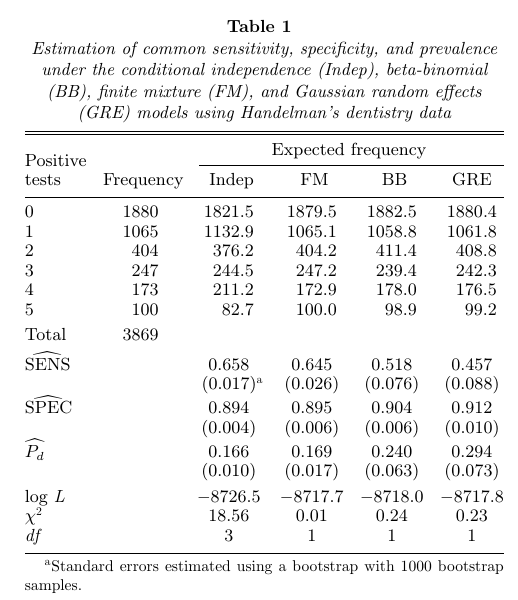
\includegraphics[scale=0.4, keepaspectratio]{./maaten}
\caption{Paper presented by Maarten Van Smeden on latent class models.}
\label{fig:ascii2}
\end{figure}

\end{frame}

%%%%%%%%%%%%%%%%%%%%%%%%%%%%%%%%%%%%%%%%%%%%%%%%%%%%%%%%%%%%%%%%%%%%%%%%%%%%%%%%%%%%%%%%%%%%%
\begin{frame}

\frametitle{The Secret Statistical Society}


\begin{figure}[h!]
\centering

\includegraphics[scale=0.3, keepaspectratio]{./stats}
\caption{Illustration of Marie-Pierre's dilemma}
\label{fig:stats}
\end{figure}

\end{frame}

%%%%%%%%%%%%%%%%%%%%%%%%%%%%%%%%%%%%%%%%%%%%%%%%%%%%%%%%%%%%%%%%%%%%%%%%%%%%%%%%%%%%%%%%%%%%%

\begin{frame}

\frametitle{Blame Copy Paste...Not Greed}


\begin{figure}[h!]
\centering
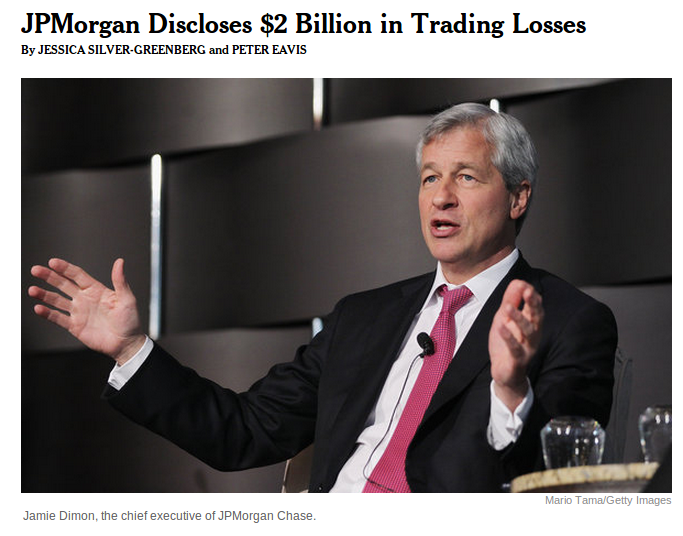
\includegraphics[scale=0.3, keepaspectratio]{./jp}
\caption{The hedging strategy operated through a series of Excel spreadsheets, which had to be \textcolor{blue}{completed manually}, by a process of \textcolor{blue}{copying and pasting} data from one spreadsheet to another}
\label{fig:jp}
\end{figure}

\end{frame}


%%%%%%%%%%%%%%%%%%%%%%%%%%%%%%%%%%%%%%%%%%%%%%%%%%%%%%%%%%%%%%%%%%%%%%%%%%%%%%%%%%%%%%%%%%%%%

\begin{frame}

\frametitle{Fabricating data}


\begin{figure}[h!]
\centering

\includegraphics[scale=0.25, keepaspectratio]{./nytimes}
\caption{Convicted of falsifying his papers and embezzling government research funds. A judge sentenced him to a suspended two-year prison term.}
\label{fig:stats}
\end{figure}

\end{frame}


%%%%%%%%%%%%%%%%%%%%%%%%%%%%%%%%%%%%%%%%%%%%%%%%%%%%%%%%%%%%%%%%%%%%%%%%%%%%%%%%%%%%%%%%%%%%%

\begin{frame}

\frametitle{Recap}

\textcolor{blue}{What are the issues here?}

\pause
\begin{enumerate}
\item Non-disclosure of ...
\item Not a requirement for journal submission
\item Copy-paste and GUI interaction
\item Lack of tools
\end{enumerate}

\pause
\textcolor{blue}{How can we improve the situation?}
\begin{enumerate}
\item Shift towards open source (e.g. \texttt{R}, \LaTeX)
\item New policies on reproducibility requirements 
\item User friendly tools
\end{enumerate}


\end{frame}


%%%%%%%%%%%%%%%%%%%%%%%%%%%%%%%%%%%%%%%%%%%%%%%%%%%%%%%%%%%%%%%%%%%%%%%%%%%%%%%%%%%%%%%%%%%%%
%%%%%%%%%%%%%%%%%%%%%%%%%%%%%%%%%%%%%%%%%%%%%%%%%%%%%%%%%%%%%%%%%%%%%%%%%%%%%%%%%%%%%%%%%%%%%
%%%%%%%%%%%%%%%%%%%%%%%%%%%%%%%%%%%%%%%%%%%%%%%%%%%%%%%%%%%%%%%%%%%%%%%%%%%%%%%%%%%%%%%%%%%%%

\lyxframeend{}\section{Tools For RR}

%%%%%%%%%%%%%%%%%%%%%%%%%%%%%%%%%%%%%%%%%%%%%%%%%%%%%%%%%%%%%%%%%%%%%%%%%%%%%%%%%%%%%%%%%%%%%
%%%%%%%%%%%%%%%%%%%%%%%%%%%%%%%%%%%%%%%%%%%%%%%%%%%%%%%%%%%%%%%%%%%%%%%%%%%%%%%%%%%%%%%%%%%%%

\lyxframeend{}\subsection{\LaTeX}

\begin{frame}[fragile]\frametitle{A powerful Typesetting system}

\begin{columns}[c] % The "c" option specifies centered vertical alignment while the "t" option is used for top vertical alignment

\column{.25\textwidth} % Left column and width
{\tiny
\begin{verbatim}
A \textbf{bold 
\textit{Hello \LaTeX}} 
to start!
\end{verbatim}
}
A \textbf{bold \textit{Hello \LaTeX}} to start !

{\tiny
\begin{verbatim}
Odds=$\left(\frac{\pi}{1-\pi} 
\right)$ 
\end{verbatim}
}

Odds=$\left( \frac{\pi}{1-\pi} \right) $




\column{.7\textwidth} % Right column and width
\small
\begin{enumerate}
%\item Used for producing scientific and mathematical documents
\item Input for \LaTeX \, is composed in plain \texttt{ASCII} using a text editor
%\item Unike Word, \LaTeX\, \textbf{\textit{is not}} What you see is what you get (WYSIWYG)
\item Although Word is useful for writing very short and simple documents, it becomes too complex or even unusable for more complicated tasks
\item Commonly needed features, like user-customized automated numbering or various automated indexes, cannot be created using Word at all
\item \LaTeX \,does require more effort and time to learn to use even for simpler tasks, but once learned, difficult tasks can be accomplished rather easily and straightforwardly
\end{enumerate}

\end{columns}

\end{frame}

%%%%%%%%%%%%%%%%%%%%%%%%%%%%%%%%%%%%%%%%%%%%%%%%%%%%%%%%%%%%%%%%%%%%%%%%%%%%%%%%%%%%%%%%%%%%%

\begin{frame}\frametitle{What is \texttt{ASCII}?}

\begin{columns}[c] % The "c" option specifies centered vertical alignment while the "t" option is used for top vertical alignment

\column{.3\textwidth} % Left column and width
\begin{figure}[h!]
\centering
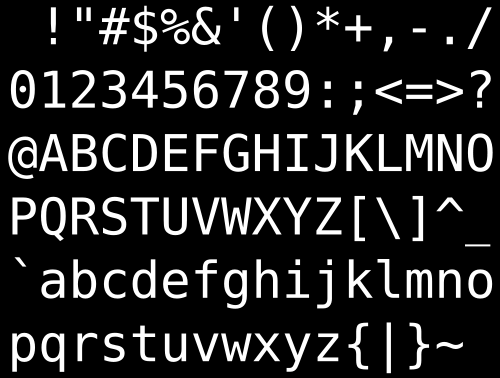
\includegraphics[scale=0.2, keepaspectratio]{./ASCIIfull}
\caption{95 printable \texttt{ASCII} characters, numbered 32 to 126. (0 to 31 \& 127 are non-printing control characters) }
\label{fig:ascii}
\end{figure}

\column{.7\textwidth} % Right column and width
\begin{enumerate}
\item When you save your document, it is saved in the form of plain text i.e in ``\texttt{ASCII}'' (the American Standard Code for Information Interchange)
\item \texttt{ASCII} is composed of 128 ($2^7$) characters: 7 binary digits for its encoding (Fig. \ref{fig:ascii})
\item An \texttt{ASCII} message will be understandable by any computer in the world. If you send such a message, you can be sure that the recipient will see precisely what you typed
\seti
\end{enumerate}
\end{columns}
\end{frame}

%%%%%%%%%%%%%%%%%%%%%%%%%%%%%%%%%%%%%%%%%%%%%%%%%%%%%%%%%%%%%%%%%%%%%%%%%%%%%%%%%%%%%%%%%%%%%

\begin{frame}\frametitle{Comparison}
\begin{columns}[c] % The "c" option specifies centered vertical alignment while the "t" option is used for top vertical alignment

\column{.45\textwidth} % Left column and width
\begin{figure}[h!]
\centering
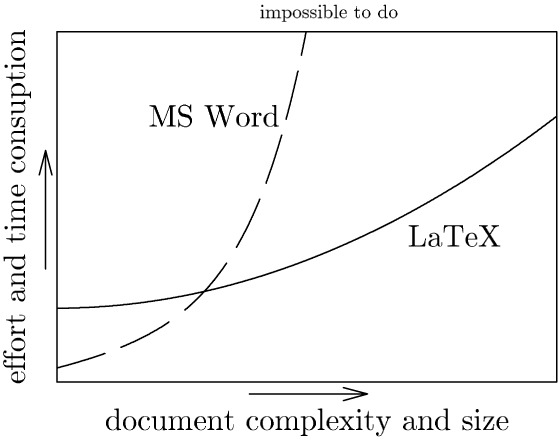
\includegraphics[scale=1, keepaspectratio]{./miktex}
\caption{Comparison}
\label{fig:word}
\end{figure}

\column{.5\textwidth} % Right column and width
\begin{itemize}
\item \LaTeX \, has a greater learning curve
\item Many tasks are very tedious or impossible (most cases) to do in MS Word or Libre Office
\end{itemize}
\end{columns}

\end{frame}

%%%%%%%%%%%%%%%%%%%%%%%%%%%%%%%%%%%%%%%%%%%%%%%%%%%%%%%%%%%%%%%%%%%%%%%%%%%%%%%%%%%%%%%%%%%%%

\begin{frame}\frametitle{The Philosophy behind \LaTeX}
\begin{columns}[c] % The "c" option specifies centered vertical alignment while the "t" option is used for top vertical alignment

\column{.45\textwidth} % Left column and width
\begin{figure}[h!]
\centering
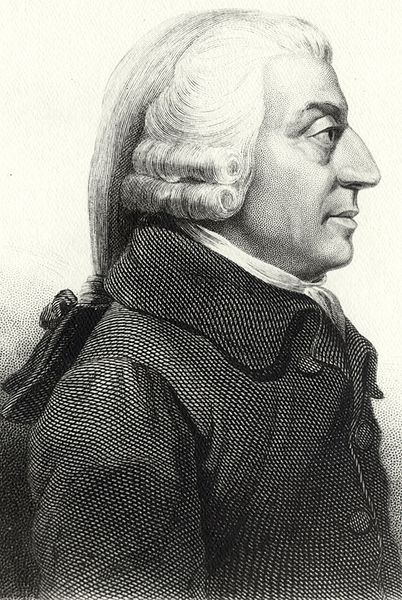
\includegraphics[scale=0.6, keepaspectratio]{./smith}
\small
\caption{Adam Smith, author of \textit{The Wealth of Nations} (1776), in which he conceptualizes the notion of the division of labour}
\label{fig:smith}
\end{figure}

\column{.5\textwidth} % Right column and width
\small
\begin{block}{Division of Labour}
Composition and logical structuring of text is the author's specific contribution to the production of a printed text. Matters such as the choice of the font family, should section headings be in bold face or small capitals? Should they be flush left or centered? Should the text be justified or not? Should the notes appear at the foot of the page or at the end? Should the text be set in one column or two? and so on, is the typesetter's business
\end{block}
\end{columns}

\end{frame}

%%%%%%%%%%%%%%%%%%%%%%%%%%%%%%%%%%%%%%%%%%%%%%%%%%%%%%%%%%%%%%%%%%%%%%%%%%%%%%%%%%%%%%%%%%%%%

\begin{frame}\frametitle{The Genius Behind \LaTeX}

\begin{figure}[h!]
\centering
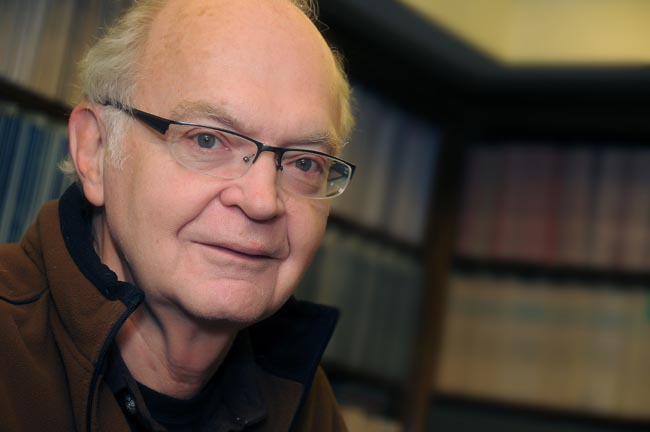
\includegraphics[scale=0.4, keepaspectratio]{./don}
\small
\caption{Donald \TeX project was started in 1978 by Donald Knuth (Stanford). He planned for 6 months, but it took him nearly 10 years to complete. Coined the term ``Literate programming'': mixture of code and text segments that are ``human'' readable. Recipient of the Turing Award (1974) and the Kyoto Prize (1996).}
\label{fig:don}
\end{figure}

\end{frame}


%%%%%%%%%%%%%%%%%%%%%%%%%%%%%%%%%%%%%%%%%%%%%%%%%%%%%%%%%%%%%%%%%%%%%%%%%%%%%%%%%%%%%%%%%%%%%
%%%%%%%%%%%%%%%%%%%%%%%%%%%%%%%%%%%%%%%%%%%%%%%%%%%%%%%%%%%%%%%%%%%%%%%%%%%%%%%%%%%%%%%%%%%%%

\lyxframeend{}\subsection{\texttt{R}}

\begin{frame}\frametitle{An Open Source Statistical Software Program}
\begin{columns}[c] % The "c" option specifies centered vertical alignment while the "t" option is used for top vertical alignment

\column{.3\textwidth} % Left column and width
\begin{figure}[h!]
\centering

\includegraphics[scale=0.6, keepaspectratio]{./Rlogo}
\small
\caption{\texttt{R} logo}
\label{fig:rlogo}
\end{figure}

\column{.7\textwidth} % Right column and width
\small
\begin{itemize}
\item You interact with \texttt{R} by explicitly writing down your steps as code
\item You cannot run analysis by clicking on dropdown menus
\item Promotes reproducibility (\href{http://cran.r-project.org/web/views/ReproducibleResearch.html}{\underline{\textcolor{blue}{CRAN task view}}})
\item \textbf{Open Source!}
\end{itemize}
\end{columns}

\end{frame}

%%%%%%%%%%%%%%%%%%%%%%%%%%%%%%%%%%%%%%%%%%%%%%%%%%%%%%%%%%%%%%%%%%%%%%%%%%%%%%%%%%%%%%%%%%%%%
%%%%%%%%%%%%%%%%%%%%%%%%%%%%%%%%%%%%%%%%%%%%%%%%%%%%%%%%%%%%%%%%%%%%%%%%%%%%%%%%%%%%%%%%%%%%%

\lyxframeend{}\subsection{Dynamic Documents with \texttt{knitr}}

\begin{frame}[fragile]

\frametitle{How to include a Figure in a \LaTeX{} document}

\begin{columns}[c] % The "c" option specifies centered vertical alignment while the "t" option is used for top vertical alignment

\column{.45\textwidth} % Left column and width
\small
\underline{\textcolor{blue}{The Tedious Way}}
\begin{verbatim}
in R:
pdf("~/cars.pdf")
plot(mtcars[ , c("disp","mpg")])
fit <- lm(mpg ~ disp , data = mtcars)
abline(fit, lwd=2)
dev.off()

then in LaTeX
\begin{figure}[h!]
\centering
\includegraphics[]{./simple}
\caption{Simple linear regression}
\label{fig:simple}
\end{figure}
\end{verbatim}


\column{.45\textwidth} % Right column and width
\begin{knitrout}\footnotesize
\definecolor{shadecolor}{rgb}{0.969, 0.969, 0.969}\color{fgcolor}\begin{figure}[]


{\centering 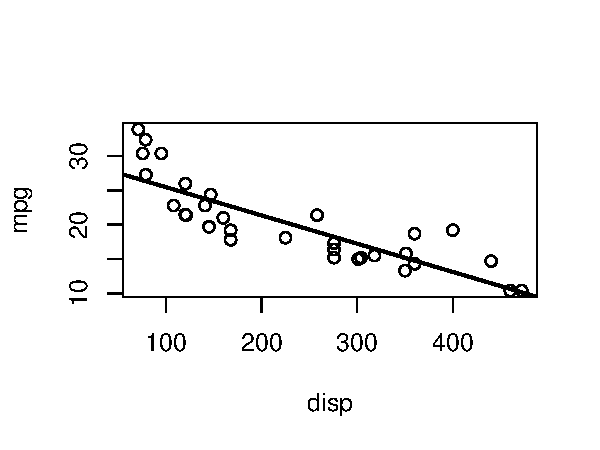
\includegraphics[width=\maxwidth]{figure/beamer-slr2} 

}

\caption[Simple linear regression]{Simple linear regression\label{fig:slr2}}
\end{figure}


\end{knitrout}

\end{columns}



\end{frame}

%%%%%%%%%%%%%%%%%%%%%%%%%%%%%%%%%%%%%%%%%%%%%%%%%%%%%%%%%%%%%%%%%%%%%%%%%%%%%%%%%%%%%%%%%%%%%

\begin{frame}
\frametitle{How to include a Figure in a \LaTeX{} document}

\begin{itemize}

\item What if the dataset changes? 
\item \href{https://github.com/sahirbhatnagar/ReproducibleResearch/blob/master/slides/finalv2.pdf}{\underline{\textcolor{blue}{ What if one observation was wrong?}}}

\end{itemize}

\end{frame}

%%%%%%%%%%%%%%%%%%%%%%%%%%%%%%%%%%%%%%%%%%%%%%%%%%%%%%%%%%%%%%%%%%%%%%%%%%%%%%%%%%%%%%%%%%%%%

\begin{frame}[fragile]
\frametitle{How to include a Figure in a \LaTeX{} document}

\begin{columns}[c] % The "c" option specifies centered vertical alignment while the "t" option is used for top vertical alignment
\column{.45\textwidth} % Left column and width
\small
\underline{\textcolor{blue}{The Dynamic Way}}
\begin{verbatim}
'<<fig.cap='Linear regression'>>=
plot(mtcars[ , c("disp","mpg")])
fit <- lm(mpg ~ disp , data = mtcars)
abline(fit, lwd=2)
'@
\end{verbatim}

\column{.45\textwidth} % Right column and width
\begin{knitrout}\footnotesize
\definecolor{shadecolor}{rgb}{0.969, 0.969, 0.969}\color{fgcolor}\begin{figure}[]


{\centering 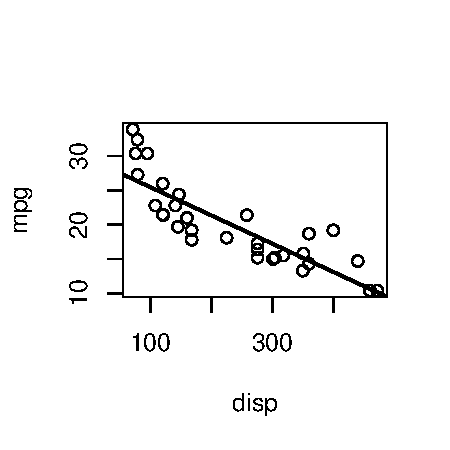
\includegraphics[width=\maxwidth]{figure/beamer-slr7} 

}

\caption[Linear regression]{Linear regression\label{fig:slr7}}
\end{figure}


\end{knitrout}

\end{columns}

\end{frame}







%%%%%%%%%%%%%%%%%%%%%%%%%%%%%%%%%%%%%%%%%%%%%%%%%%%%%%%%%%%%%%%%%%%%%%%%%%%%%%%%%%%%%%%%%%%%%

\begin{frame}[fragile]
\frametitle{\texttt{R} + \LaTeX = \texttt{knitr} (Yihui Xie (2013))}
\begin{knitrout}\footnotesize
\definecolor{shadecolor}{rgb}{0.969, 0.969, 0.969}\color{fgcolor}\begin{kframe}
\begin{alltt}
\hlstd{(x} \hlkwb{=} \hlkwd{rnorm}\hlstd{(}\hlnum{20}\hlstd{))}  \hlcom{# create some random numbers}
\end{alltt}
\begin{verbatim}
##  [1]  0.14496  0.43832  0.15319  1.08494  1.99954 -0.81188
##  [7]  0.16027  0.58589  0.36009 -0.02531  0.15088  0.11008
## [13]  1.35968 -0.32699 -0.71638  1.80977  0.50840 -0.52746
## [19]  0.13272 -0.15594
\end{verbatim}
\begin{alltt}
\hlkwd{boxplot}\hlstd{(x)}
\hlkwd{hist}\hlstd{(x,} \hlkwc{main} \hlstd{=} \hlstr{""}\hlstd{,} \hlkwc{col} \hlstd{=} \hlstr{"blue"}\hlstd{,} \hlkwc{probability} \hlstd{=} \hlnum{TRUE}\hlstd{)}
\hlkwd{lines}\hlstd{(}\hlkwd{density}\hlstd{(x),} \hlkwc{col} \hlstd{=} \hlstr{"red"}\hlstd{)}
\end{alltt}
\end{kframe}

{\centering 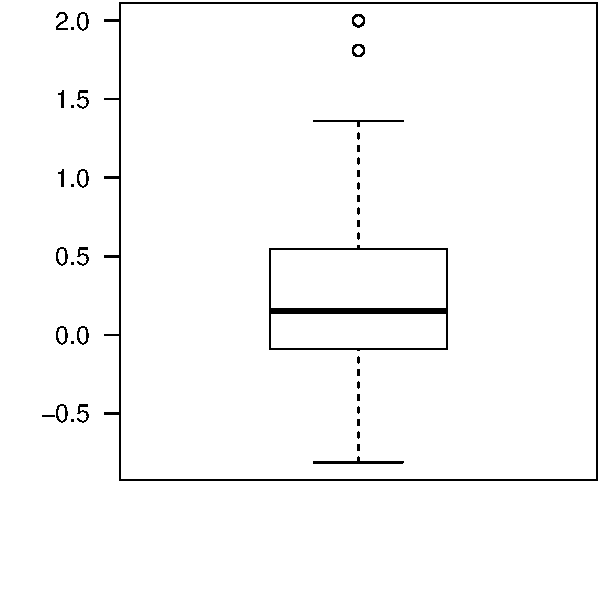
\includegraphics[width=.45\linewidth]{figure/beamer-boring-plots1} 
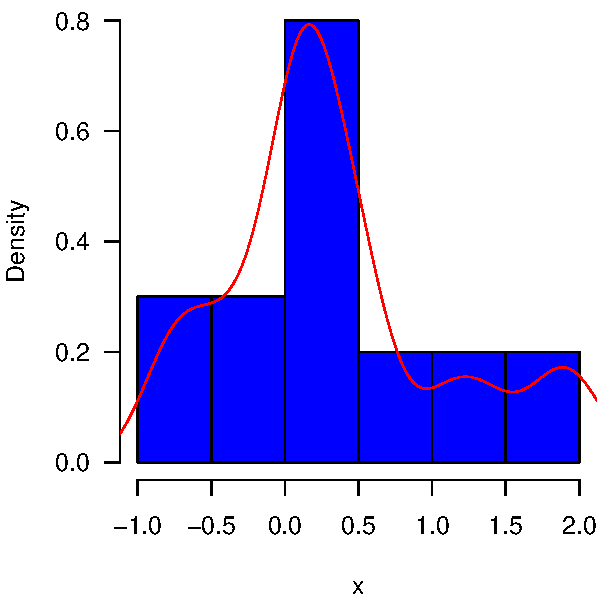
\includegraphics[width=.45\linewidth]{figure/beamer-boring-plots2} 

}



\end{knitrout}


\end{frame}

%\href{run:../Biostat-2009-Peng-405-8.pdf}{biostat}



%%%%%%%%%%%%%%%%%%%%%%%%%%%%%%%%%%%%%%%%%%%%%%%%%%%%%%%%%%%%%%%%%%%%%%%%%%%%%%%%%%%%%%%%%%%%%

\begin{frame}[fragile]
\frametitle{The possibilities are endless}

\textcolor{blue}{Pros}

\begin{itemize}
\item Highly customizable for \href{https://github.com/sahirbhatnagar/ReproducibleResearch/blob/master/examples/knit_expand/mtcars.Rnw}{\underline{\textcolor{blue}{ repetitive}}}  \href{https://github.com/sahirbhatnagar/ReproducibleResearch/blob/master/examples/knit_expand/template.Rnw}{\underline{\textcolor{blue}{ tasks}}}
\item Easily extendible to \href{https://github.com/sahirbhatnagar/ReproducibleResearch/blob/master/examples/markdown/mwe.Rmd}{\underline{\textcolor{blue}{ Markdown documents}}} (Gruber 2004) 
\item Interactive presentations via \href{http://sahirbhatnagar.github.io/RR}{\underline{\textcolor{blue}{ \texttt{Slidify}}}} (Vaidyanathan 2013)
\item Interactive \href{https://github.com/sahirbhatnagar/prostate}{\underline{\textcolor{blue}{ web applications}}} to present results
\item Avoids error prone copy-paste
\item Ensures reproducibility
\item Allows for caching (think big data)
\item You can focus more time on methods and analysis
\end{itemize}

\pause

\textcolor{blue}{Cons}

\begin{itemize}
\item Brute force brings us instant gratification 
\end{itemize}


\end{frame}


%%%%%%%%%%%%%%%%%%%%%%%%%%%%%%%%%%%%%%%%%%%%%%%%%%%%%%%%%%%%%%%%%%%%%%%%%%%%%%%%%%%%%%%%%%%%%

\begin{frame}
\frametitle{RR Workflow}

\begin{figure}[h!]
\centering
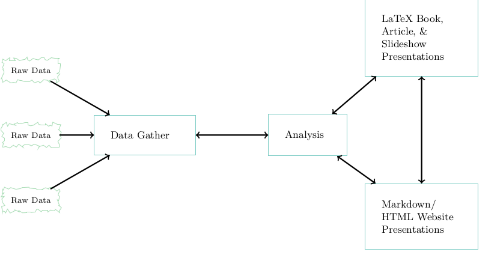
\includegraphics[scale=0.6, keepaspectratio]{./rrfig}
\small
\caption{An example workflow. Notice the direction of the arrows. (\emph{Gandrud 2014})}
\label{fig:rlogo}
\end{figure}


\end{frame}


%%%%%%%%%%%%%%%%%%%%%%%%%%%%%%%%%%%%%%%%%%%%%%%%%%%%%%%%%%%%%%%%%%%%%%%%%%%%%%%%%%%%%%%%%%%%%
%%%%%%%%%%%%%%%%%%%%%%%%%%%%%%%%%%%%%%%%%%%%%%%%%%%%%%%%%%%%%%%%%%%%%%%%%%%%%%%%%%%%%%%%%%%%%

\lyxframeend{}\subsection{Version Control with GitHub}

\begin{frame}
\frametitle{A Motivating Quote}

\begin{center}
\large
\emph{``It's week 3... So it must be binomial.''} - J.A. Hanley
\end{center}


\end{frame}

%%%%%%%%%%%%%%%%%%%%%%%%%%%%%%%%%%%%%%%%%%%%%%%%%%%%%%%%%%%%%%%%%%%%%%%%%%%%%%%%%%%%%%%%%%%%%

\begin{frame}
\frametitle{Storing Your Files in the Cloud: GitHub}

\underline{\textcolor{blue}{What is GitHub?}}
\begin{itemize}
\item An interface and a cloud hosting service built on top of the Git version control system
\item Git does the version control
\item GitHub allows you to store the data remotely
\end{itemize}


\end{frame}


%%%%%%%%%%%%%%%%%%%%%%%%%%%%%%%%%%%%%%%%%%%%%%%%%%%%%%%%%%%%%%%%%%%%%%%%%%%%%%%%%%%%%%%%%%%%%

\begin{frame}
\frametitle{Storing Your Files in the Cloud: GitHub}

\underline{\textcolor{blue}{Why use GitHub?}}
\begin{enumerate}

\item \textbf{Storage and Access}
\begin{itemize}
\item Makes projects accessible on a fully featured website
\item Can create and host a website to present results 
\end{itemize}

\vspace{0.2in}
\pause
\item \textbf{Collaboration}
\begin{itemize}
\item Keeps meticulous records of who contributed what to a project
\item ``Issues'' tracker
\item Each project can host a wiki
\item Anyone can suggest changes to files in a public repository
\end{itemize}

\vspace{0.2in}
\pause
\item \textbf{Version Control}
\begin{itemize}
\item Can easily revert back to any change you make
\item Previous file versions in Dropbox disappear after 30 days. GitHub stores them indefinetly
\item Identifies difference between two documents and lets you reconcile them
\end{itemize}

\end{enumerate}


\end{frame}

%%%%%%%%%%%%%%%%%%%%%%%%%%%%%%%%%%%%%%%%%%%%%%%%%%%%%%%%%%%%%%%%%%%%%%%%%%%%%%%%%%%%%%%%%%%%%

\begin{frame}
\frametitle{Storing Your Files in the Cloud: GitHub}

\underline{\textcolor{blue}{The main point here is to avoid:}}

\begin{center}
manuscript\_v1.2.3\_July\_2013\_sahir.tex
\end{center}

or 

\begin{center}
data\_analysis\_and\_cleaning\_v2.R
\end{center}

\end{frame}


%%%%%%%%%%%%%%%%%%%%%%%%%%%%%%%%%%%%%%%%%%%%%%%%%%%%%%%%%%%%%%%%%%%%%%%%%%%%%%%%%%%%%%%%%%%%%

\begin{frame}
\frametitle{Open Source}

\begin{figure}[h!]
\centering
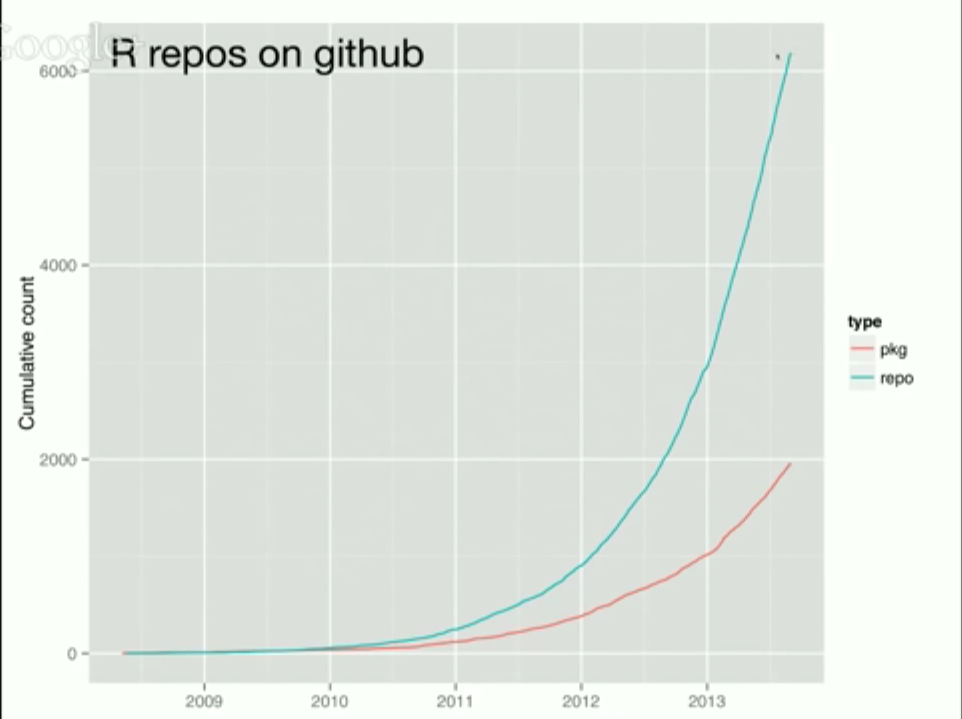
\includegraphics[scale=0.25, keepaspectratio]{./rgit}
\small
\caption{\texttt{R} projects and packages hosted on GitHub (\emph{Wickham 2013})}
\label{fig:med3}
\end{figure}


\end{frame}



%%%%%%%%%%%%%%%%%%%%%%%%%%%%%%%%%%%%%%%%%%%%%%%%%%%%%%%%%%%%%%%%%%%%%%%%%%%%%%%%%%%%%%%%%%%%%
%%%%%%%%%%%%%%%%%%%%%%%%%%%%%%%%%%%%%%%%%%%%%%%%%%%%%%%%%%%%%%%%%%%%%%%%%%%%%%%%%%%%%%%%%%%%%
%%%%%%%%%%%%%%%%%%%%%%%%%%%%%%%%%%%%%%%%%%%%%%%%%%%%%%%%%%%%%%%%%%%%%%%%%%%%%%%%%%%%%%%%%%%%%

\lyxframeend{}\section{Is the juice worth the squeeze?}

%%%%%%%%%%%%%%%%%%%%%%%%%%%%%%%%%%%%%%%%%%%%%%%%%%%%%%%%%%%%%%%%%%%%%%%%%%%%%%%%%%%%%%%%%%%%%
%%%%%%%%%%%%%%%%%%%%%%%%%%%%%%%%%%%%%%%%%%%%%%%%%%%%%%%%%%%%%%%%%%%%%%%%%%%%%%%%%%%%%%%%%%%%%

\lyxframeend{}\subsection{Journals}

\begin{frame}
\frametitle{Medicine}

\begin{figure}[h!]
\centering

\includegraphics[scale=0.3, keepaspectratio]{./med}
\small
\caption{Annals of Internal Medicine (\emph{Liane et al. 2007})}
\label{fig:med}
\end{figure}


\end{frame}


%%%%%%%%%%%%%%%%%%%%%%%%%%%%%%%%%%%%%%%%%%%%%%%%%%%%%%%%%%%%%%%%%%%%%%%%%%%%%%%%%%%%%%%%%%%%%

\begin{frame}
\frametitle{Bioconductor}

\begin{figure}[h!]
\centering

\includegraphics[scale=0.3, keepaspectratio]{./bioc}
\small
\caption{Bioconductor (\emph{Gentleman and Lang 2004})}
\label{fig:med2}
\end{figure}


\end{frame}


%%%%%%%%%%%%%%%%%%%%%%%%%%%%%%%%%%%%%%%%%%%%%%%%%%%%%%%%%%%%%%%%%%%%%%%%%%%%%%%%%%%%%%%%%%%%%

\begin{frame}
\frametitle{Biostatistics}

\begin{figure}[h!]
\centering

\includegraphics[scale=0.3, keepaspectratio]{./peng}
\small
\caption{Biostatistics (\emph{Peng 2009})}
\label{fig:med3}
\end{figure}


\end{frame}



%%%%%%%%%%%%%%%%%%%%%%%%%%%%%%%%%%%%%%%%%%%%%%%%%%%%%%%%%%%%%%%%%%%%%%%%%%%%%%%%%%%%%%%%%%%%%
%%%%%%%%%%%%%%%%%%%%%%%%%%%%%%%%%%%%%%%%%%%%%%%%%%%%%%%%%%%%%%%%%%%%%%%%%%%%%%%%%%%%%%%%%%%%%

\lyxframeend{}\subsection{CRAN}

\begin{frame}
\frametitle{CRAN has a dedicated Task View for RR}

\begin{center}
\large
\href{http://cran.r-project.org/web/views/}{\underline{\textcolor{blue}{ CRAN Task Views}}}
\end{center}


\end{frame}

%%%%%%%%%%%%%%%%%%%%%%%%%%%%%%%%%%%%%%%%%%%%%%%%%%%%%%%%%%%%%%%%%%%%%%%%%%%%%%%%%%%%%%%%%%%%%

\begin{frame}
\frametitle{\emph{Biostatistics} requirements for RR}


\begin{enumerate}
\item data analysis script
\item other code
\item data
\item script for results used in paper
\item \texttt{knitr} file (\texttt{.Rnw})
\item resulting \texttt{.tex} file from compiling with \texttt{knitr}
\item bib\TeX file
\end{enumerate}


\end{frame}



%%%%%%%%%%%%%%%%%%%%%%%%%%%%%%%%%%%%%%%%%%%%%%%%%%%%%%%%%%%%%%%%%%%%%%%%%%%%%%%%%%%%%%%%%%%%%
%%%%%%%%%%%%%%%%%%%%%%%%%%%%%%%%%%%%%%%%%%%%%%%%%%%%%%%%%%%%%%%%%%%%%%%%%%%%%%%%%%%%%%%%%%%%%

\lyxframeend{}\subsection{Summary}


\begin{frame}[c]
\frametitle{The Main Idea}

\begin{center}
\begin{block}{Jon Claerbout, Geophysicist at Stanford, (1995)}
\emph{``An article about computational science in a scientific publication is \textbf{not} the scholarship itself, it is merely \textbf{advertising} of the scholarship. The actual scholarship is the \textbf{complete software development environment} and the \textbf{complete set of instructions} which generated the figures''}
\end{block}
\end{center}


\end{frame}












\begin{frame}
\frametitle{If you can only take away one thing from today's discussion...}

\[ \textrm{Reproducibility} \propto \frac{1}{\textrm{copy paste}}  \]


\end{frame}








\lyxframeend{}\subsection{References}
\begin{frame}[allowframebreaks]
\frametitle<presentation>{References}    
\bibliographystyle{amsalpha}
\nocite{ams}
\nocite{laine}
\nocite{peng}
\nocite{ny}
\nocite{london}
\nocite{gandrud}
\nocite{yihui}

\bibliography{biblio.bib}
%\bibliography{biblio.bib}
\end{frame}

\end{document}
